\documentclass{standalone}
\usepackage{tikz}
\usetikzlibrary{arrows.meta}

\begin{document}
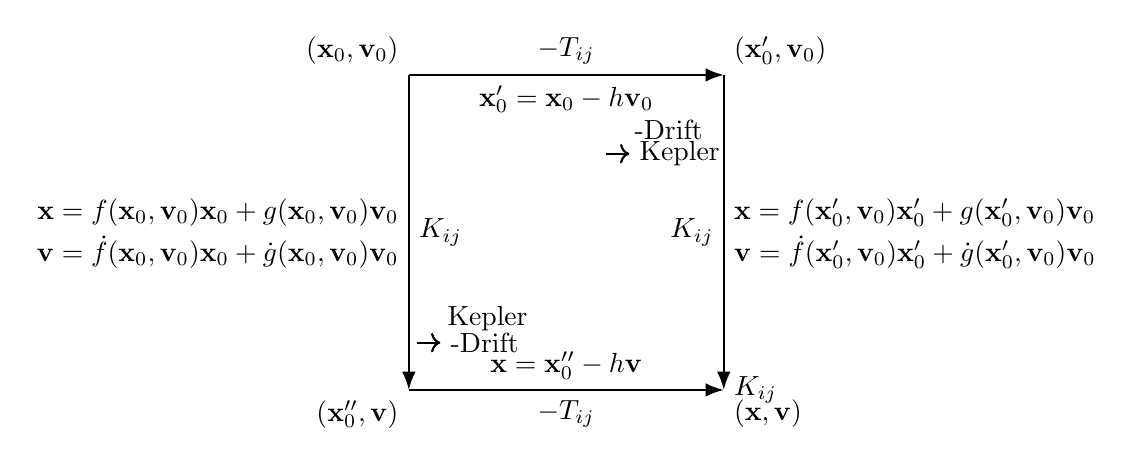
\begin{tikzpicture}

\draw[thick,-Latex] (0,0) node[above left] {$(\mathbf{x}_0,\mathbf{v}_0)$}-- (2,0) node[above]{$-T_{ij}$} node[below]{$\mathbf{x}_0^\prime = \mathbf{x}_0-h\mathbf{v}_0$} -- (4,0) node[above right]{$(\mathbf{x}_0^\prime,\mathbf{v}_0)$};
\draw[thick,-Latex] (4,0) -- (4,-1.75)  node[right]{$\mathbf{x} = f(\mathbf{x}_0^\prime,\mathbf{v}_0) \mathbf{x}_0^\prime + g(\mathbf{x}_0^\prime,\mathbf{v}_0) \mathbf{v}_0$} -- (4,-2)node[left]{$K_{ij}$}-- (4,-2.25) node[right]{$\mathbf{v} = \dot f(\mathbf{x}_0^\prime,\mathbf{v}_0) \mathbf{x}_0^\prime + \dot g(\mathbf{x}_0^\prime,\mathbf{v}_0) \mathbf{v}_0$} -- (4,-4) node[right]{$K_{ij}$};
\draw[thick,-Latex] (0,0) -- (0,-1.75) node[left]{$\mathbf{x} = f(\mathbf{x}_0,\mathbf{v}_0) \mathbf{x}_0+ g(\mathbf{x}_0,\mathbf{v}_0) \mathbf{v}_0$} -- (0,-2)node[right]{$K_{ij}$} -- (0,-2.25)  node[left]{$\mathbf{v} = \dot f(\mathbf{x}_0,\mathbf{v}_0) \mathbf{x}_0+ \dot g(\mathbf{x}_0,\mathbf{v}_0) \mathbf{v}_0$}-- (0,-4) node[below left]{$(\mathbf{x}_0^{\prime\prime},\mathbf{v})$};
\draw[thick,-Latex] (0,-4) -- (2,-4) node[below]{$-T_{ij}$} node[above]{$\mathbf{x} = \mathbf{x}_0^{\prime\prime}-h\mathbf{v}$} -- (4,-4) node[below right]{$(\mathbf{x},\mathbf{v})$};
\node[draw=none] at (3.3,-0.7) {-Drift};
\draw[thick,->] (2.5,-1.0) -- (2.8,-1.0) node[right]{Kepler};
\node[draw=none] at (1.0,-3.1) {Kepler};
\draw[thick,->] (0.1,-3.4) -- (0.4,-3.4) node[right]{-Drift};
\end{tikzpicture}

\end{document}
